\documentclass{beamer}
\usetheme{CambridgeUS}
\usecolortheme{beaver}
\usepackage{amsmath,amssymb,enumerate,amsthm}
\usepackage{bm}

\newcommand{\profile}{\bm{v}}%(complete) profile
\newcommand{\pprofile}{{\bm{p}}}%partial profile
\newcommand{\w}{\bm{w}}
\newcommand{\W}{\mathcal{W}}
\newcommand{\Co}{\mathcal{C}}
\newcommand{\pw}{W}%our knowledge about the weights
\newcommand{\strat}[1]{\emph{#1}}
\newcommand{\ppref}{\succ^\text{p}}%partial pref
\newcommand{\pprefeq}{\succeq^\text{p}}%partial pref
\newcommand{\pref}{\succ}% pref
\DeclareMathOperator{\Regret}{Regret}
\DeclareMathOperator{\SCORE}{Score}
\DeclareMathOperator{\PMR}{PMR}
\DeclareMathOperator{\MR}{MR}
\DeclareMathOperator{\MMR}{MMR}

\newcommand*{\icimg}[1]{%
	\raisebox{-.3\baselineskip}{%
		\includegraphics[
		height=\baselineskip,
		width=\baselineskip,
		keepaspectratio,
		]{#1}%
	}%
}

\newcommand*{\icarr}[1]{%
	\raisebox{-0.4\baselineskip}{%
		\includegraphics[
		height=2.5\baselineskip,
		width=3\baselineskip,
		keepaspectratio,
		]{#1}%
	}%
}

\makeatletter
\defbeamertemplate*{title page}{mydefault}[1][]
{
	\vbox{}
	\vfill
	\begin{centering}

%{\usebeamercolor[fg]{titlegraphic}\inserttitlegraphic\par}
		\begin{beamercolorbox}{titlegraphic}
				\usebeamerfont{titlegraphic}\inserttitlegraphic
		\end{beamercolorbox}%
			\vskip1em\par	
		\begin{beamercolorbox}[rounded=true, center, shadow=true, sep=8pt,#1]{title}
			\usebeamerfont{title}\inserttitle\par%
			\ifx\insertsubtitle\@empty%
			\else%
			\vskip0.5em%
			{\usebeamerfont{subtitle}\usebeamercolor[fg]{subtitle}\insertsubtitle\par}%
			\fi%     
		\end{beamercolorbox}%
		\vskip1em\par
		\begin{beamercolorbox}[sep=8pt,center,#1]{author}
			\usebeamerfont{author}\insertauthor
		\end{beamercolorbox}
		\begin{beamercolorbox}[sep=8pt,center,#1]{institute}
			\usebeamerfont{institute}\insertinstitute
		\end{beamercolorbox}
		\begin{beamercolorbox}[sep=8pt,center,#1]{date}
			\usebeamerfont{date}\insertdate
		\end{beamercolorbox}\vskip0.5em
		\begin{beamercolorbox}[sep=8pt,center,#1]{logo}
			\usebeamerfont{titlegraphic}\insertlogo
		\end{beamercolorbox}%
	\end{centering}
	\vfill
}
\setbeamertemplate{title page}[mydefault]
\makeatother



\titlegraphic{
\includegraphics[width=50mm]{logo_dauphine} \hspace*{5.5cm} 
\includegraphics[width=7mm]{cnrs}}
\title[Elicitation of Incomplete Preferences]{Simultaneous Elicitation of Committee and \\ Voters' Preferences}
\institute[]{$^1$ LAMSADE, Université Paris-Dauphine, Paris, France \\ $^2$ LIP6, Sorbonne Universit\'e, Paris, France}
\author[B. Napolitano, O. Cailloux, P. Viappiani]{B. Napolitano$^1$, O. Cailloux$^1$ and P. Viappiani$^2$}
%
%\title[Elicitation and Explanation in Social Choice]{Elicitation and Explanation in Social Choice Theory}
%%\subtitle{Proposal: ``Elicitation and Explanation for Voting Rules''}
%\author[Beatrice Napolitano]{\textbf{Beatrice Napolitano} \\
%	Supervisors: Remzi Sanver, Olivier Cailloux}
\date[RJCIA 2019]{{\small RJCIA 2019} \\ 
\includegraphics[width=35mm]{LOGO_LAMSADE} }

\usepackage{tikz}
\usepackage{amsmath}
\usepackage{graphicx}

\definecolor{darkred}{rgb}{0.8,0,0}

\begin{document}

\beamertemplatenavigationsymbolsempty

\begin{frame}[plain]
\maketitle
\end{frame}

\addtocounter{framenumber}{-1}


\section{Setting}
\subsection{Scenario}

\begin{frame}
\frametitle{Scenario}
%\framesubtitle{Robust Winner Determination}
%	\textbf{Setting}: Two kind of players
\textbf{Setting}: Incompletely specified profile and positional scoring rule
\begin{figure}
	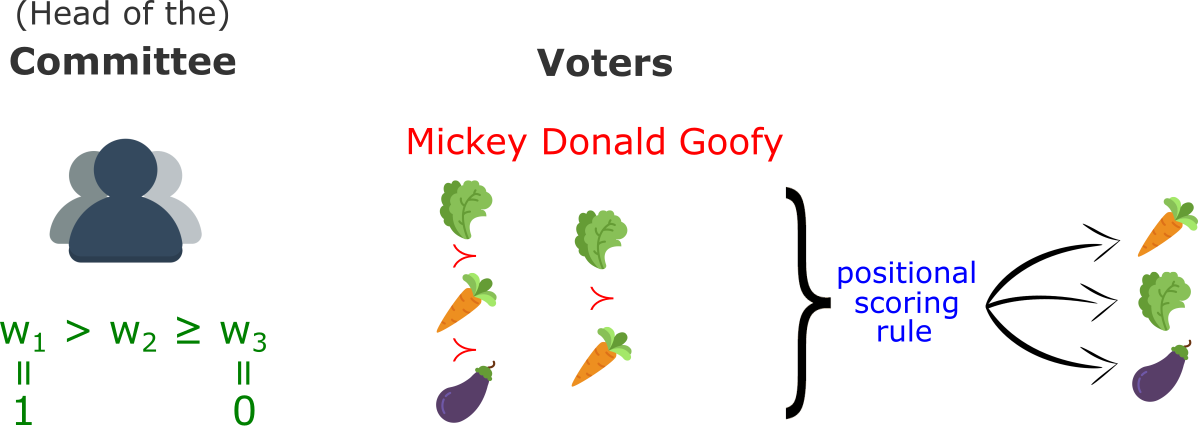
\includegraphics[scale=0.35]{setting3.png}
	%		\caption{.}
	%		\label{fig:b1}
\end{figure}
\textbf{Goal}: Development of an incremental elicitation protocol based on minimax regret 
\end{frame}
%\addtocounter{framenumber}{-1}
%\begin{frame}
%	\frametitle{Scenario}
%	\textbf{Setting}: Incompletely specified profile and positional scoring rule
%	\begin{figure}
%		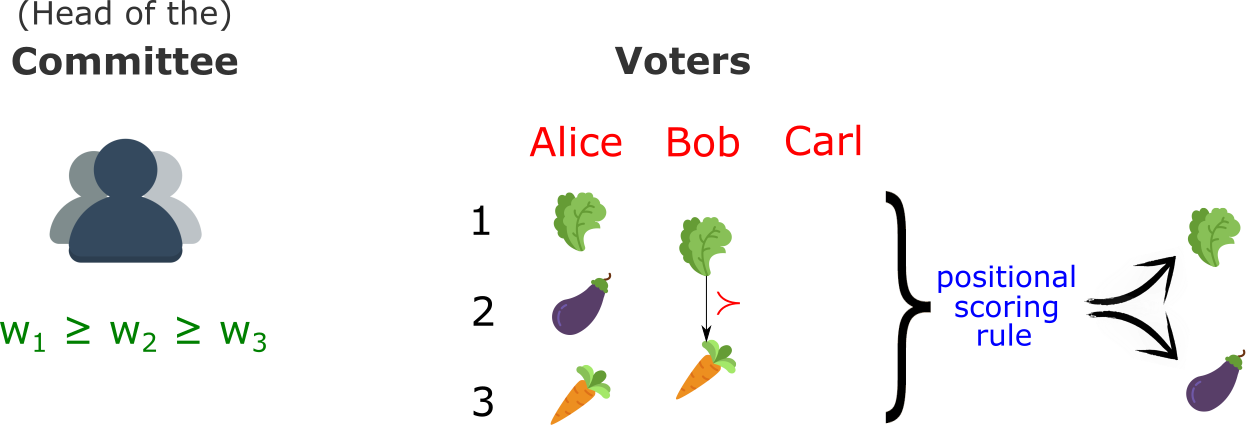
\includegraphics[scale=0.35]{set2.png}
%%		\caption{.}
%%		\label{fig:b1}
%	\end{figure}
%	\textbf{Goal}: Development of an incremental elicitation protocol based on minimax regret 
%\end{frame}

\subsection{Pairwise Max Regret Computation}
\begin{frame}
	\frametitle{Pairwise Max Regret Computation}
	The computation of the regret of selecting \icimg{salad.png} as a winner instead of choosing \icimg{aubergine.png} can be seen as a game in which an adversary both:
	\begin{itemize}
		\item \textbf{chooses a complete profile}\\
		\medskip
		\begin{center}
			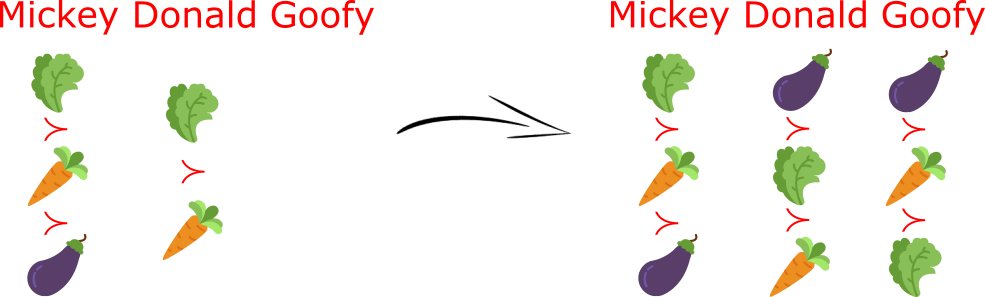
\includegraphics[scale=0.35]{completion4.png}
		\end{center}
		
		\item \textbf{chooses a feasible weight vector}\\
		\medskip
		\centerline{\color{red}$\mathbf{(1,?,0)}$ \icarr{arrow.png} \color{red}$\mathbf{(1,0,0)}$}
	\end{itemize}
	\medskip
	in order to maximize the difference of scores
\end{frame}


%\addtocounter{framenumber}{-1}


\bibliographystyle{plain}
\bibliography{biblio} 
%given a combination of axioms we want to find an outcome that doesn't satisfy them, and we would do that for several reasons:
%-querying the user, depending of her answer we might infer her preferences over the set of axioms;
%-proving that a set of axioms is not valid giving a counter-example;


%A method for automatically proving impossibility theorems in the area of ranking sets of objects has already been implemented (Geist \& Endriss, 2011). It:



\end{document}